% TU Delft beamer template
% Author: Erwin Walraven (initial version was created by Maarten Abbink)
% Delft Universiy of Technology

\documentclass{beamer}
\usepackage[english]{babel}
\usepackage{calc}
\usepackage[absolute,overlay]{textpos}
\usepackage{graphicx}
\usepackage{subfig}
\usepackage{amsmath}
\usepackage{amsfonts}
\usepackage{amsthm}
\usepackage{mathtools}
\usepackage{comment}
\usepackage{MnSymbol,wasysym}
\usepackage{physics}
\usepackage{tikz}
\usetikzlibrary{quantikz}

\setbeamertemplate{navigation symbols}{} % remove navigation symbols
\mode<presentation>{\usetheme{tud}}

% BIB SETTINGS
\usepackage[backend=bibtex,firstinits=true,maxnames=30,maxcitenames=20,url=false,style=authoryear]{biblatex}
\bibliography{bibfile}
\setlength\bibitemsep{0.3cm} % space between entries in the reference list
\renewcommand{\bibfont}{\normalfont\scriptsize}
\setbeamerfont{footnote}{size=\tiny}
\renewcommand{\cite}[1]{\footnote<.->[frame]{\fullcite{#1}}}


\title[]{Learning with quantum kernels: early applications to material damage prediction}
\institute[]{Delft University of Technology, The Netherlands}
\author{Giorgio Tosti Balducci}
%\date{}

\begin{document}
{
\setbeamertemplate{footline}{\usebeamertemplate*{minimal footline}}
\frame{\titlepage}
}

{\setbeamertemplate{footline}{\usebeamertemplate*{minimal footline}}

}

\begin{frame}
    \frametitle{The team}

    \begin{itemize}
        \item Boyang Chen - \emph{Aerospace Engineering}
        \item Matthias M\"{o}ller - \emph{Applied Mathematics}
        \item Marc Gerritsma - \emph{Aerospace Engineering}
        \item me - \emph{Aerospace Engineering}
    \end{itemize}

    \vspace{1.5cm}
    \centering
    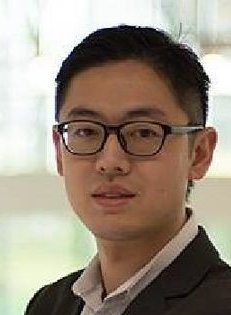
\includegraphics[width=.15\textwidth]{pics/boyang.jpeg}
    \hspace{.5cm}
    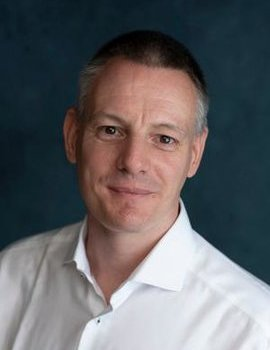
\includegraphics[width=.16\textwidth]{pics/matthias.jpeg}
    \hspace{.5cm}
    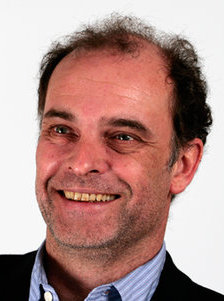
\includegraphics[width=.16\textwidth]{pics/marc.jpeg}
    \hspace{.5cm}
    
\includegraphics[width=.2\textwidth]{pics/giorgio.jpeg}
        
\end{frame}

\begin{frame}
    \frametitle{Quantum machine learning}
    \framesubtitle{Some informal definitions}

    \begin{block}{\textbf{Quantum-enhanced machine learning}}
        Quantum computation to speed-up classical machine learning operations.

        \ \\
        \emph{Example}: SVM with quantum linear systems solver algorithm
    \end{block}

    \begin{block}{\textbf{Machine learning in quantum feature spaces}}
        Information is \emph{encoded} into quantum states and classical algorithms find the optimal model
    \end{block}

    \ \\
    \pause
    \footnotesize
    \emph{Note}: not all quantum machine learning is done on quantum computers. QML can also mean to use classical machine learning for quantum mechanics.


\end{frame}

\begin{frame}
    \frametitle{Quantum machine learning in the near term}

    Quantum-enhanced ML gives provable speed-up, but requires \textbf{fault-tolerant hardware}. However \dots

    \ \\
    \pause
    \begin{minipage}{\textwidth}
        \centering
        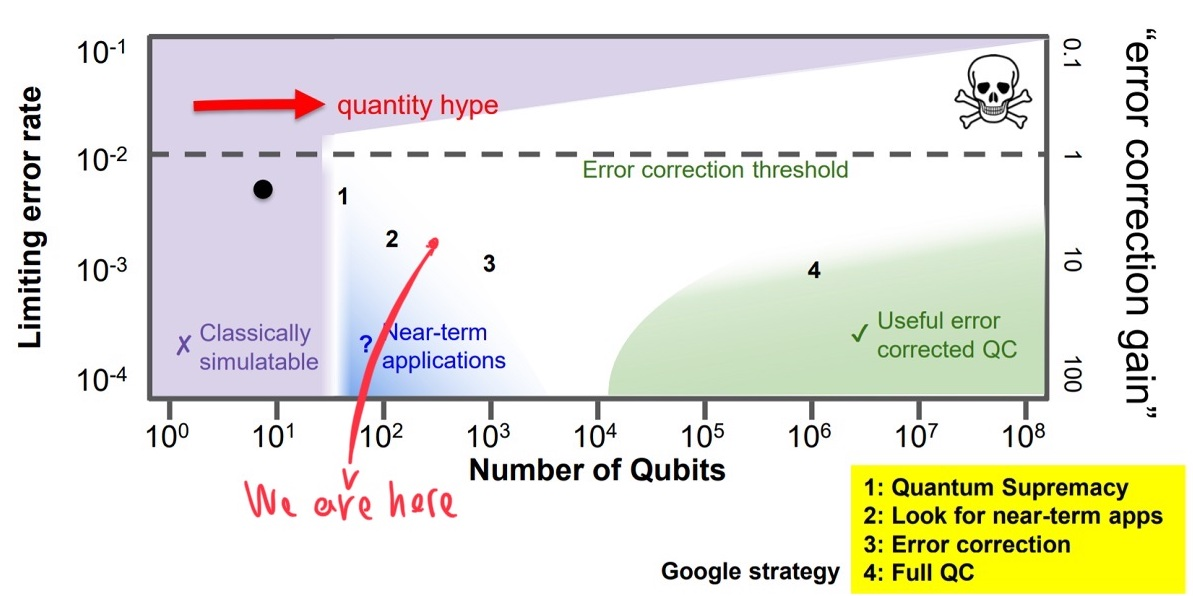
\includegraphics[width=.7\textwidth]{pics/google-quality-quantity-chart-here.jpeg}

        \scalebox{.2}{Source: https://www.hpcwire.com/2018/04/26/google-frames-quantum-race-as-two-dimensional/}
        
        \ \\
        \color{red} Quantum-enhanced ML is not viable in the near term.
      \end{minipage}


\end{frame}

\begin{frame}
    \frametitle{ML in quantum feature spaces}

    Can we learn data patterns that are \emph{hard to learn classically}?

    \ \\
    \pause
    \begin{minipage}{.45\textwidth}
        \centering
        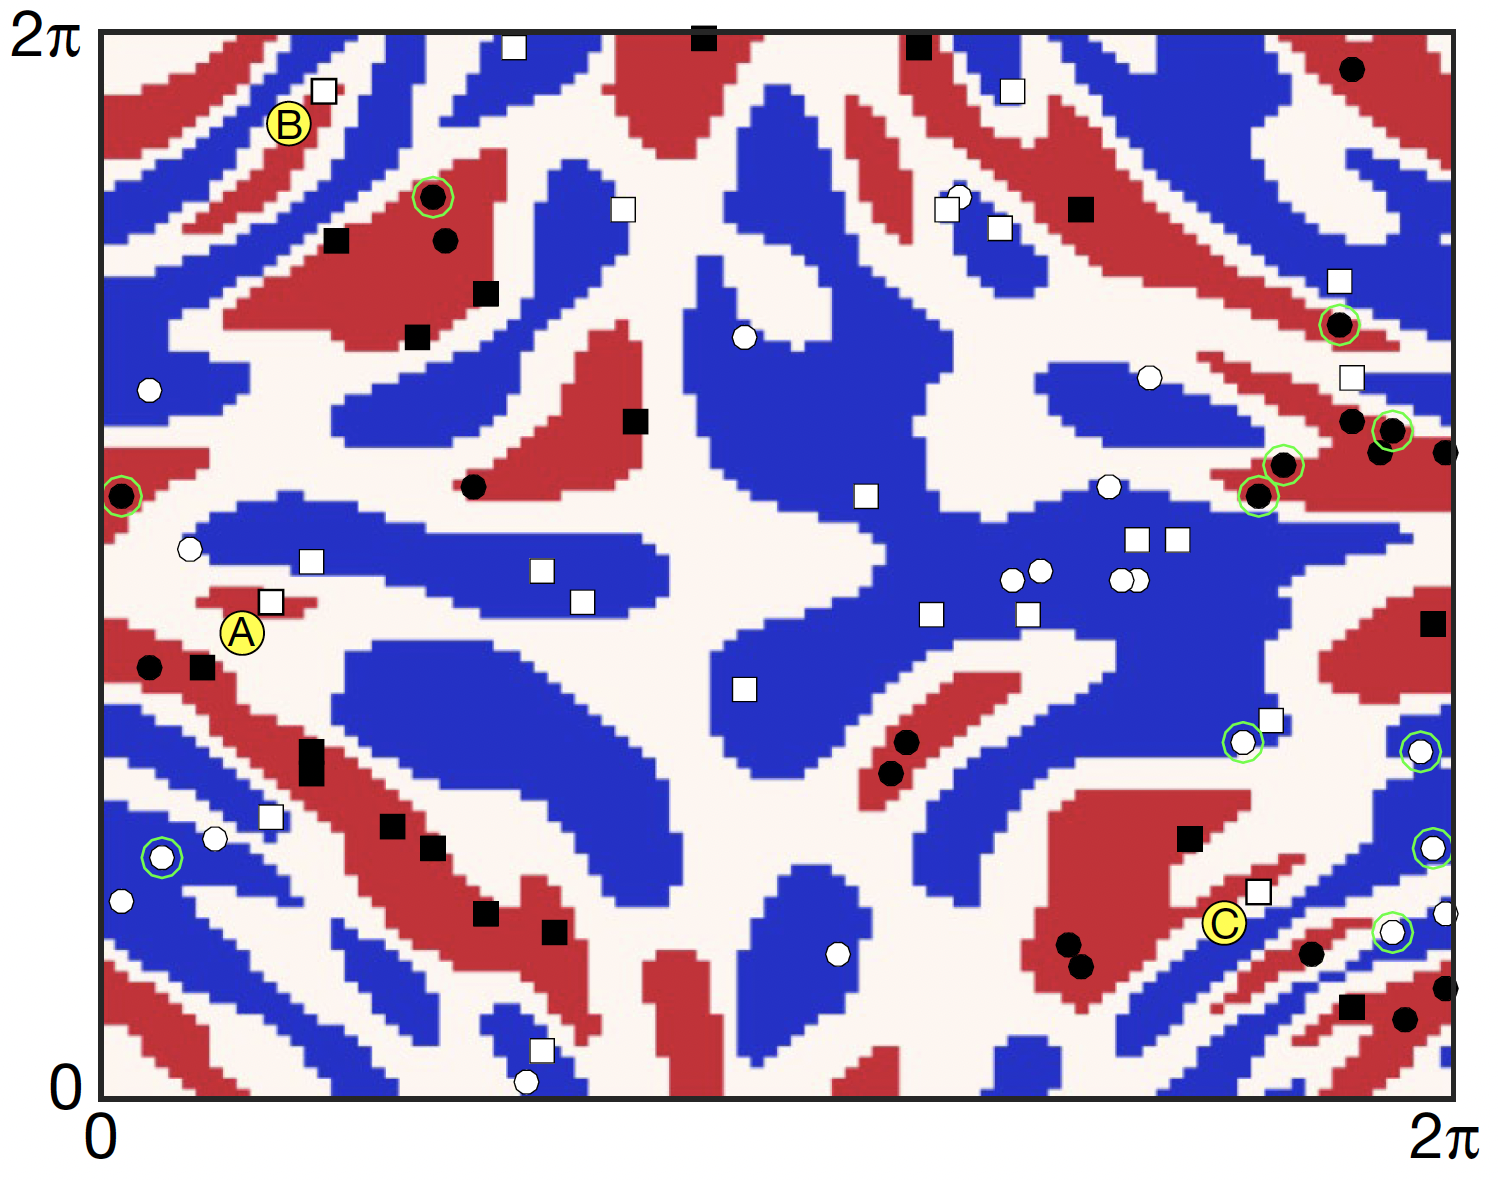
\includegraphics[width=.8\textwidth]{pics/havlicek-data.png}

        \scalebox{.2}{Source: Havlicek \emph{et al.}, 2019, Nature Physics}
    \end{minipage}
    \begin{minipage}{.45\textwidth}
        \small
        Data generated from a `quantum model' such to be hard to access classically.

    \end{minipage}
    
    \begin{minipage}{.45\textwidth}
        \centering
        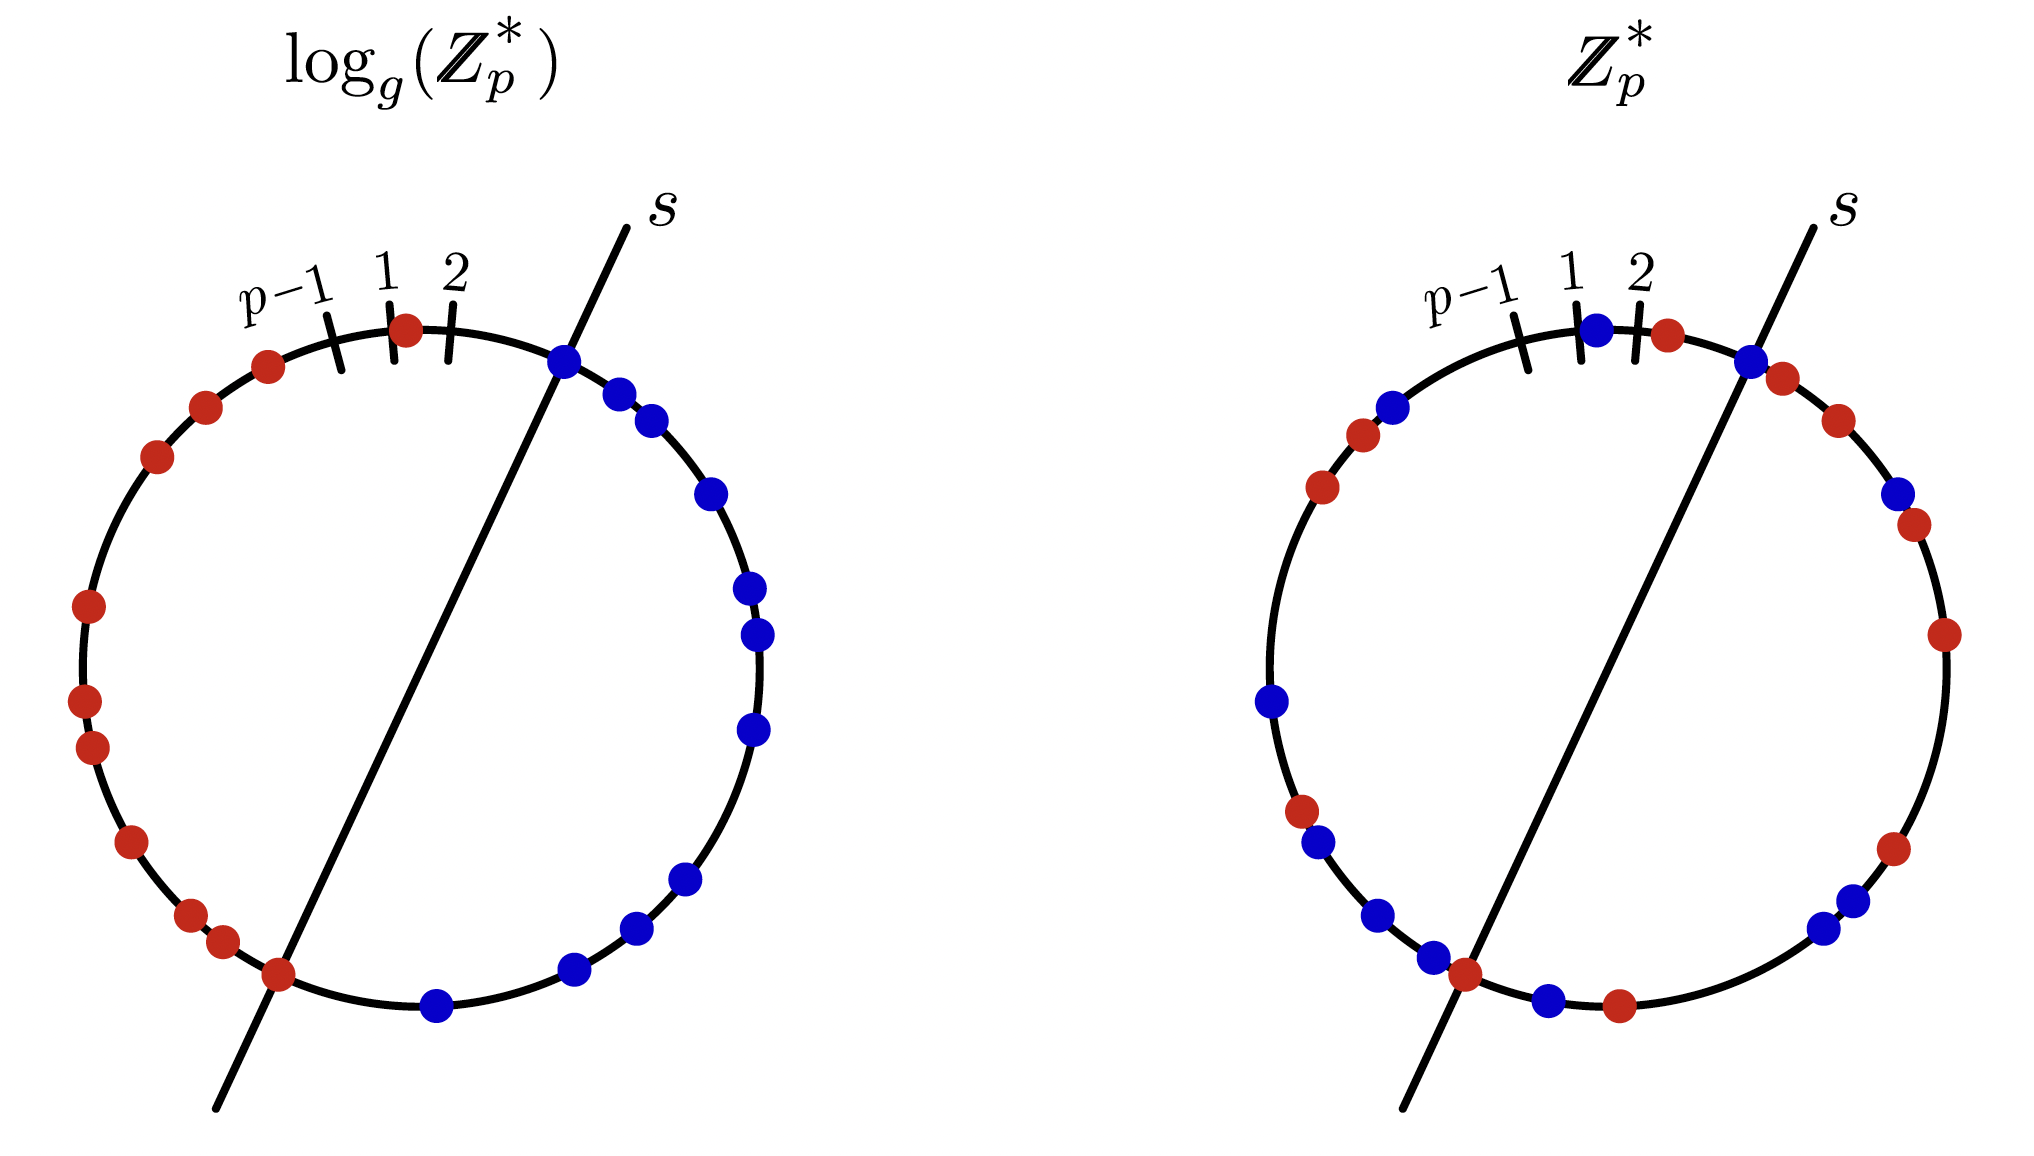
\includegraphics[width=.8\textwidth]{pics/liu-temme-data.png}

        \scalebox{.2}{Source: Liu \emph{et al.}, 2020, arXiv:2010.02174}
    \end{minipage}
    \begin{minipage}{.45\textwidth}
        \small
        Data labelled by discrete loagarithm over a group generated by a large prime number.

        Classically hard to compute, but efficient with Shor's quantum algorithm.
    \end{minipage}

\end{frame}

\begin{frame}
    \frametitle{ML in quantum feature spaces}

    \centering
    \color{red} Are there \emph{real world} datasets that are classically hard to classify, but `understandable' for quantum computers?

\end{frame}

\begin{frame}
    \frametitle{Maximum margin classifier}
    \begin{minipage}{.45\textwidth}
        Assume that the data is linearly separable (perhaps with some noise)

        \ \\
        Model:
            \[y=\text{sgn}\left( \langle \mathbf{w},\, \mathbf{x}\rangle + b \right)\]
        
    \end{minipage}
    \begin{minipage}{.45\textwidth}
        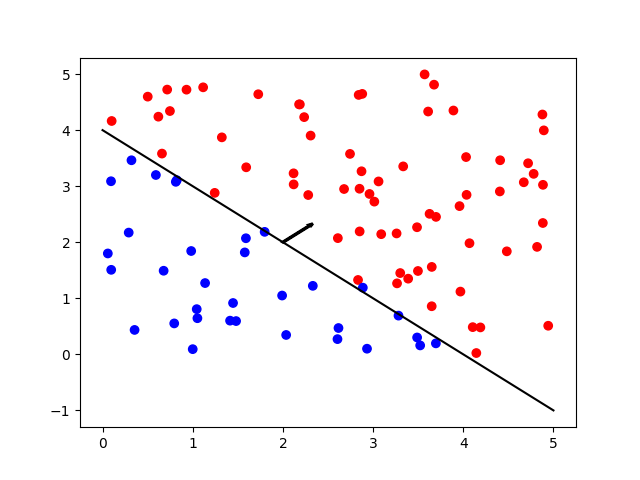
\includegraphics[width=\textwidth]{pics/lin-sep.png}
    \end{minipage}
    
    \begin{block}{Support vector machine, primal form (\emph{maximum geometric-margin classifier})}
        \begin{align*}
            \min_{w,b} & \quad \frac{1}{2}\norm{\mathbf{w}}^2 \\
            \mathrm{s.t.} & \quad y^{(i)}\left( \mathbf{w}^\top \mathbf{x}^{(i)} + b \right) \geq 1, \quad i=1,\dots, m
        \end{align*}

    \end{block}

    \end{frame}

    \begin{frame}
        \frametitle{Maximum margin classifier}
    
        What if the data is \emph{not} linearly separable? We can introduce a feature map $\phi\left( x \right)$

        \begin{center}
        \begin{minipage}{.4\textwidth}
            \centering
            \includegraphics[width=.8\textwidth]{pics/circle-data-2-feats-eps-converted-to.pdf}
        \end{minipage}
        \begin{minipage}{.48\textwidth}
            \centering
            \includegraphics[width=\textwidth]{pics/circle-data-3-feats-eps-converted-to.pdf}
        \end{minipage}
        \[
            \xrightarrow[\phi\left( x \right)=\left\{x_1,\, x_2,\, 0.5 \left( x_1^2 + x_2^2 \right)\right\}]{}
            \]
        \end{center}

        Model: $y=\text{sgn}\left( \langle \mathbf{w},\, \phi\left( \mathbf{x} \right)\rangle + b \right) $
    
    \end{frame}

    \begin{frame}
        \frametitle{Kernels}

        \begin{block}{Representer theorem}
            The vector that expresses the optimal separating hyperplane in feature space is a linear combination of feature vectors.
            \[
                \mathbf{w} = \sum_{i=1}^{N^\prime \leq N} \alpha_i \phi\left( \mathbf{x}_i \right)
            \]
            
        \end{block}

        \pause
        So we can rewrite our model as
        \[y=\text{sgn}\left( \sum_{i=1}^{N^\prime \leq N} \alpha_i \langle \phi\left( \mathbf{x}_i \right),\, \phi\left( \mathbf{x} \right)\rangle + b \right),\]
        which is \emph{linear in the feature space}.

        \ \\
        The quantity $k\left( \mathbf{x}, \mathbf{x}^\prime \right)=\langle \phi\left( \mathbf{x} \right),\, \phi\left( \mathbf{x}^\prime \right)\rangle$ is called the \emph{kernel} induced by the feature map $\phi$.
    
    
    \end{frame}

    \begin{frame}
        \frametitle{Kernel trick}
    
        If we find an efficient explicit formula for the kernel, we don't need to compute the feature map directly and we can \emph{implicitly} compute distances and classify in the feature space.

        \ \\
        \small
        \begin{exampleblock}{\small Example: quadratic kernel}
            \begin{align*}
                \mathbf{x} &= \left( x_1,\, x_2 \right)^\top\\
                \phi\left( \mathbf{x} \right) &= \left( x_1^2,\, \sqrt{2}x_1x_2,\, x_2^2 \right)^\top\\
                k\left( \mathbf{x}, \mathbf{x}^\prime \right) &= \langle \phi\left( \mathbf{x} \right),\, \phi\left( \mathbf{x}^\prime \right)\rangle \\
                &= \left( x_1 x_1^\prime + x_2 x_2^\prime \right)^2\\
                &= \langle \mathbf{x},\, \mathbf{x}^\prime\rangle^2
            \end{align*}

            i.e. the kernel can be computed in the original space of data.
        \end{exampleblock}
    
    \end{frame}

    
    \begin{frame}
        \frametitle{Quantum kernels}

        \begin{minipage}{.4\textwidth}
            \footnotesize
            In terms of quantum states, we can encode $\mathbf{x}$ into a unitary operator $U\left( \mathbf{x} \right)$. This creates $\ket{\phi\left( \mathbf{x} \right)} = U\left( \mathbf{x} \right) \ket{0}$
            
        \end{minipage}
        \begin{minipage}{.4\textwidth}
            \centering
            \begin{quantikz}
                \lstick[wires=4]{$\ket{0}^{\otimes n}$} & \gate[wires=4]{U\left( \mathbf{x} \right)} & \qw \rstick[wires=4]{$\ket{\phi\left( \mathbf{x} \right)}$} \\
                &  &\qw \\
                &  &\qw \\
                &  &\qw
            \end{quantikz}
        \end{minipage}
        
        \pause
        \begin{minipage}{.4\textwidth}
            \footnotesize
            Defining $\rho\left( \mathbf{x} \right) = \ketbra{\mathbf{x}}{\mathbf{x^\prime}}$, the \emph{quantum kernel} $k\left( \mathbf{x}, \mathbf{x}^\prime \right) = \mathrm{Tr}\left\{ \rho\left( \mathbf{x} \right)\rho\left( \mathbf{x^\prime} \right) \right\}$ implicitly accesses the $4^n$-dimensional complex space
        \end{minipage}
        \begin{minipage}{.4\textwidth}
            \centering
            \begin{quantikz}
                \lstick[wires=4]{$\ket{0}^{\otimes n}$} & \gate[wires=4]{U\left( \mathbf{x} \right)} & \gate[wires=4]{U^\dagger\left( \mathbf{x^\prime} \right)} & \meter{} \\
                &  &  & \meter{}\\
                &  &  & \meter{}\\
                &  &  & \meter{}
            \end{quantikz}
        \end{minipage}
        
    \end{frame}
    
    \begin{frame}
        \frametitle{Material damage prediction}
        \begin{minipage}{.45\textwidth}
            \small
            \begin{itemize}
                \item Failure criteria are models of material failure. They generally come from semi-empirical relations (data + physics)
                \item They are effectively \emph{classification problems}, where the decision boundary is the \emph{failure envelope}
            \end{itemize}
        \end{minipage}
        \begin{minipage}{.45\textwidth}
            \centering
            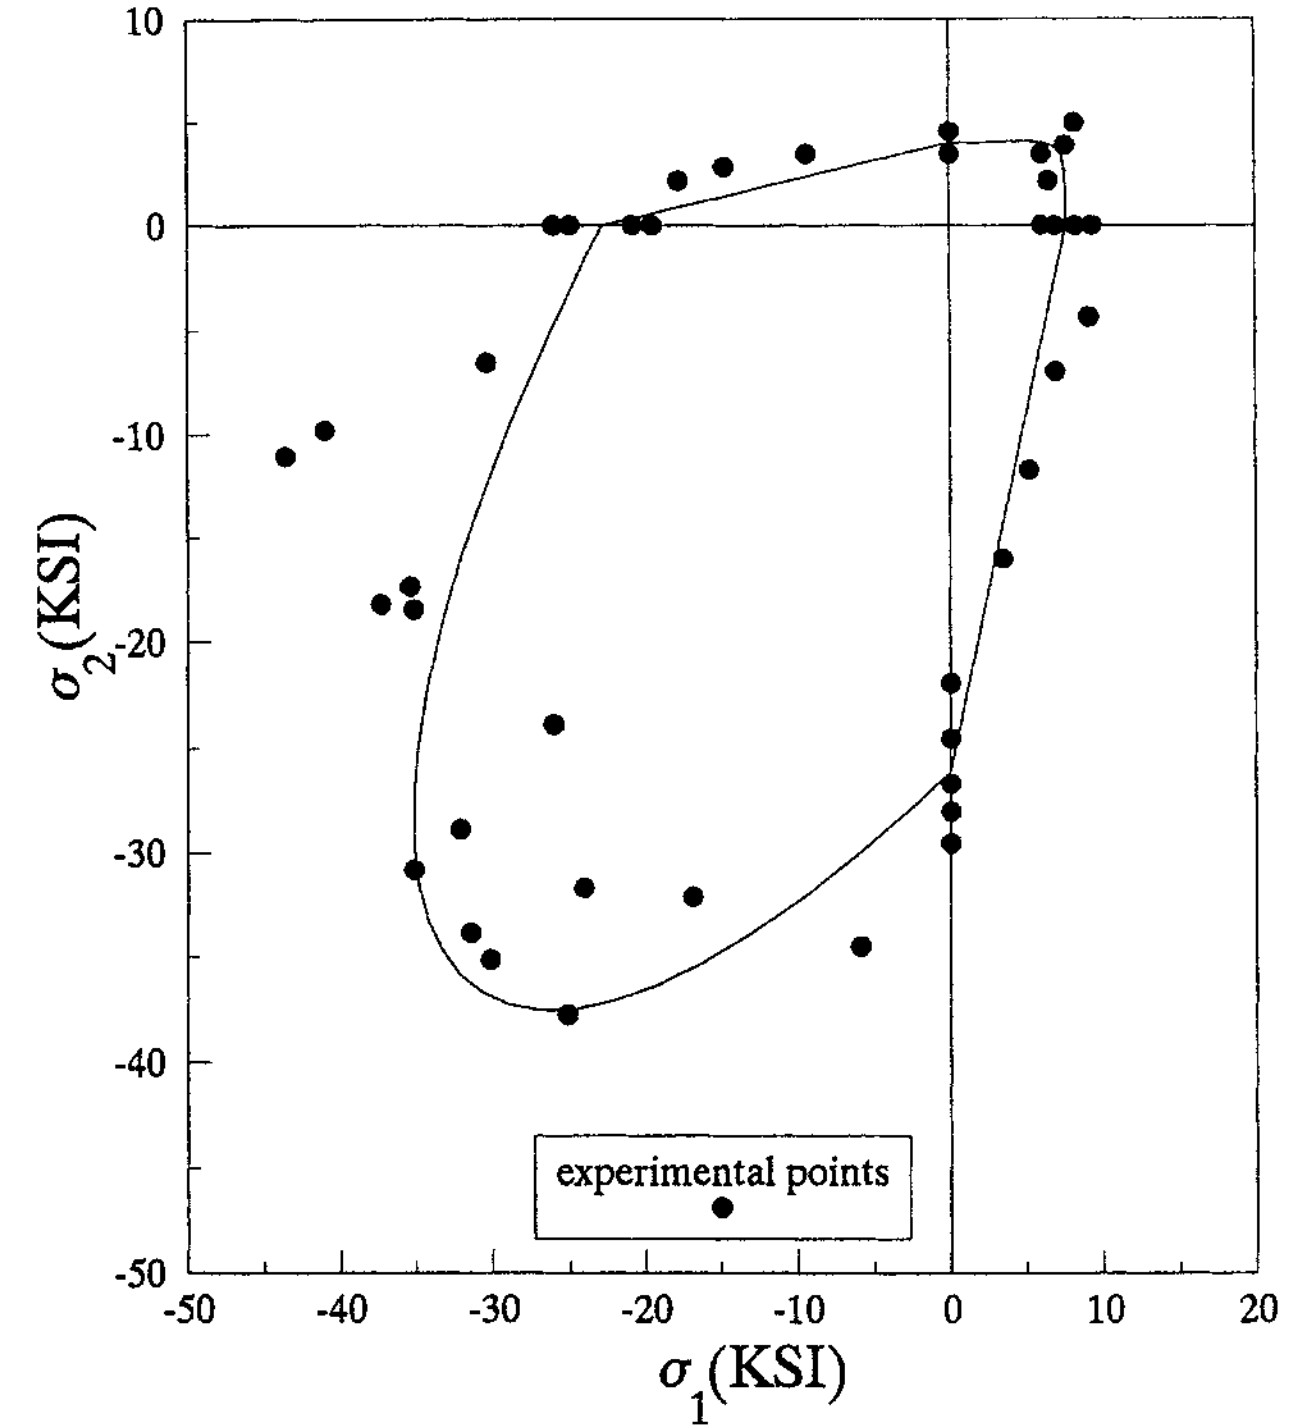
\includegraphics[width=\textwidth]{pics/fail-env-example.png}

            \scalebox{.2}{Source: Echaabi \emph{et al.}, 1996, Polymer Composites}
        \end{minipage}
        
    \end{frame}
    
    \begin{frame}
        \frametitle{Von Mises criterion}
        \framesubtitle{A \texttt{hello, world!} example in material damage prediction}
        
        \begin{tikzpicture}[overlay,remember picture]
            \node[left=0.2cm] at (current page.25){
                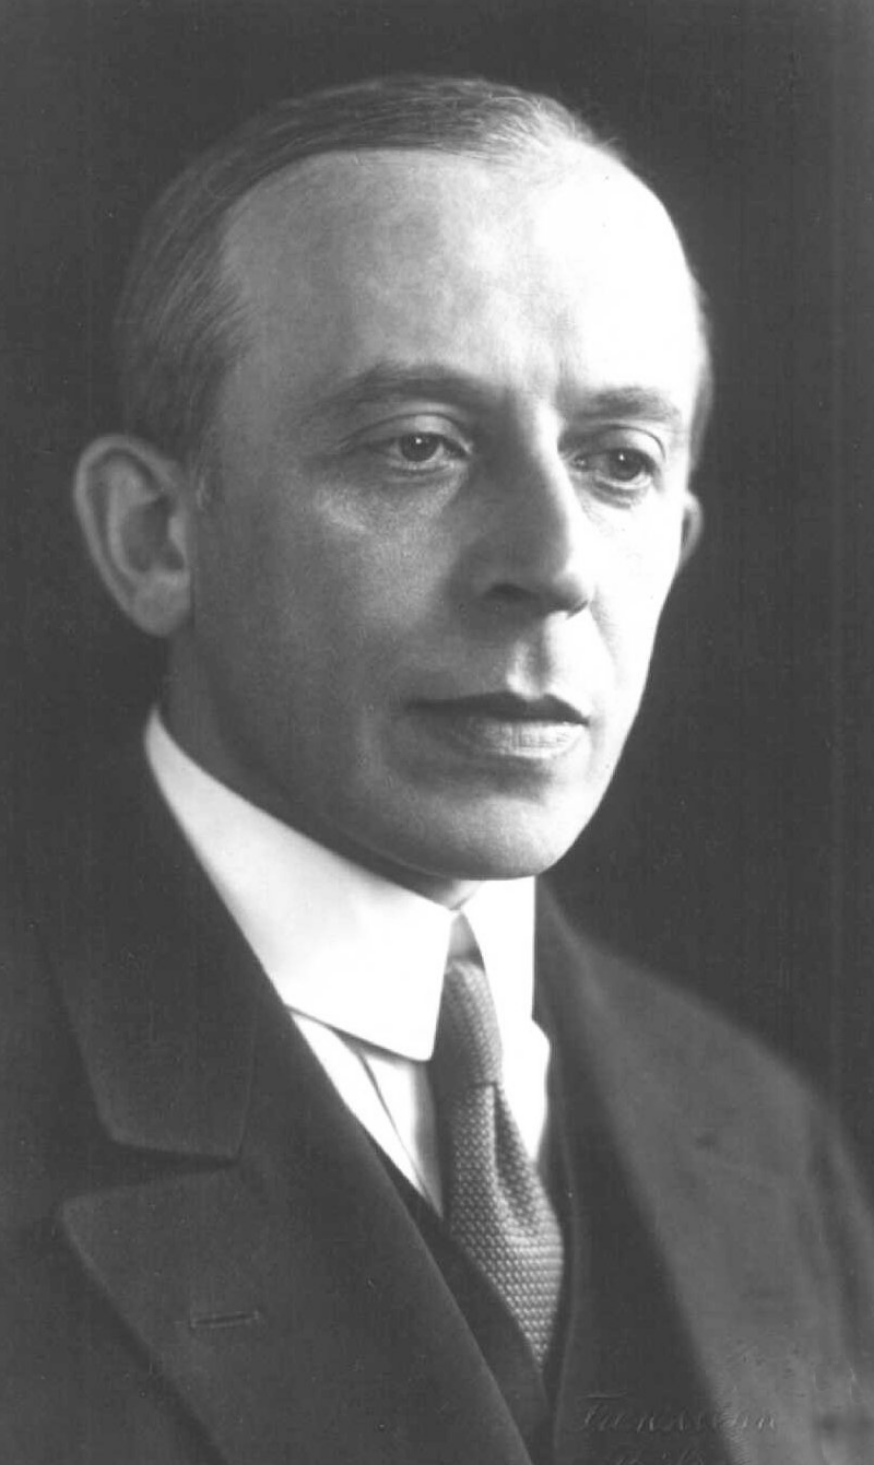
\includegraphics[width=2cm]{pics/von-mises-portrait.jpeg}
            };
        \end{tikzpicture}
        
        \begin{minipage}{.45\textwidth}
            \centering
            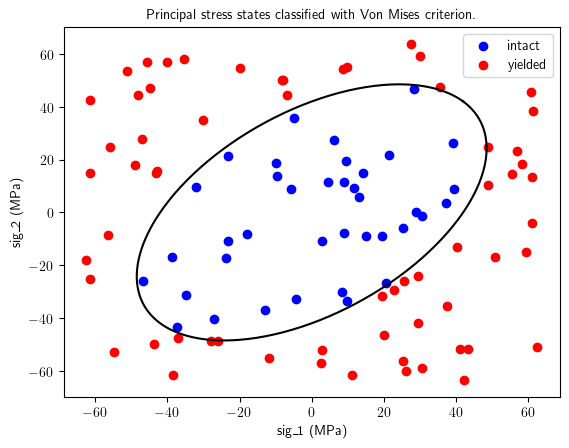
\includegraphics[width=\textwidth]{pics/vm-data-envelope.png}
            
        \end{minipage}
        \hspace{1cm}
        \begin{minipage}{.3\textwidth}
            \[
                \sigma_1^2 + \sigma_2^2 -\sigma_1\sigma_2 - \sigma_y^2 = 0
            \]
            \pause
            `Analytic' feature map and kernel:
            \begin{gather*}
                \phi\left( \mathbf{x} \right) = \left( x_1^2,\, x_2^2,\, x_1 x_2 \right)\\
                k\left( \mathbf{x}, \mathbf{x}^\prime \right) = \langle \phi\left( \mathbf{x} \right), \phi\left( \mathbf{x}^\prime \right) \rangle
            \end{gather*}
        \end{minipage}
        
        
    \end{frame}
    
    \begin{frame}
        \frametitle{Von Mises criterion}
        \framesubtitle{Classification with classical quadratic kernel}
        
        \centering
        \[
            k\left( \mathbf{x}, \mathbf{x}^\prime \right) = \left( \gamma\langle \mathbf{x}, \mathbf{x}^\prime \rangle + r \right)^2
        \]

        \begin{minipage}{.45\textwidth}
            \centering
            Kernel matrix
            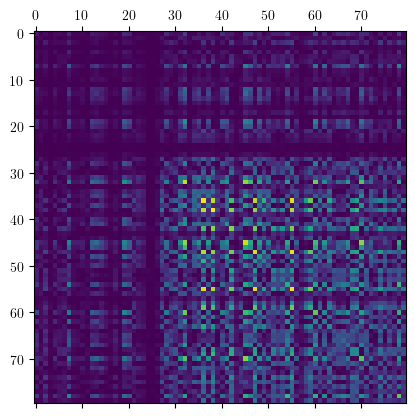
\includegraphics[width=\textwidth]{pics/quad-kernel-matrix.png}
        \end{minipage}
        \begin{minipage}{.45\textwidth}
            \centering
            Failure envelope
            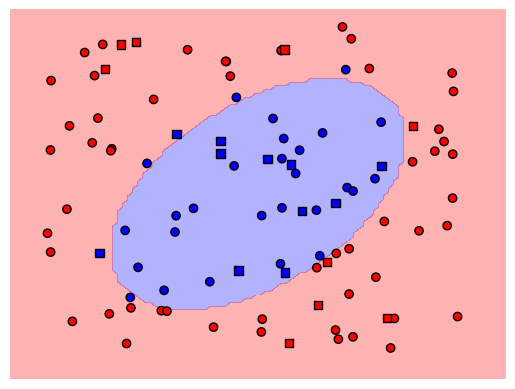
\includegraphics[width=\textwidth]{pics/quad-kernel-envelope.png}
        \end{minipage}
    \end{frame}
    
    \begin{frame}
        \frametitle{Von Mises criterion}
        \framesubtitle{Using a quantum `quadratic' kernel}
        
        Strictly speaking, if we `simply' encode $\mathbf{x}$ as the quantum state $\ket{x}$, it seems that we recover the quadratic kernel.
        
        \centering
        \[
            \phi\left( \mathbf{x} \right) = \ket{x} \longrightarrow k\left( \mathbf{x}, \mathbf{x}^\prime \right) = \abs{\mathbf{x}^\dagger \mathbf{x}^\prime}^2
        \]

        \pause
        \begin{minipage}{.3\textwidth}
            However, the kernel matrix does not show any class separation\dots
        \end{minipage}
        \begin{minipage}{.6\textwidth}
            \centering
            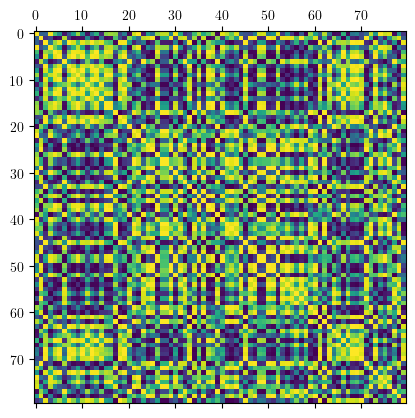
\includegraphics[width=.6\textwidth]{pics/amp-enc-kernel-matrix.png}
        \end{minipage}  
        
    \end{frame}

    \begin{frame}
        \frametitle{Von Mises criterion}
        \framesubtitle{Using a quantum `quadratic' kernel}
    
        Reason: normalization to quantum states completely confuses the data

        \ \\
        \pause
        \centering
        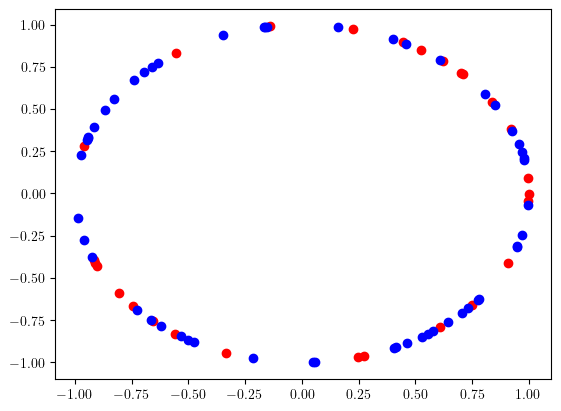
\includegraphics[width=.6\textwidth]{pics/vm-data-2d-normalized.png}
    
    \end{frame}
    
    \begin{frame}
        \frametitle{Von Mises criterion}
        \framesubtitle{Using the same kernel in a 4-dimensional space of unit vectors}
        
        \begin{minipage}{.45\textwidth}
            Hack: add a 3rd dimension and normalize on a semi-sphere.
            
            \[
                \phi\left( \mathbf{x} \right) = \left( x_1,\, x_2,\, 1,\, 0 \right)^\top / \norm*{\mathbf{x}}
                \]
        \end{minipage}
        \begin{minipage}{.45\textwidth}
            \centering
            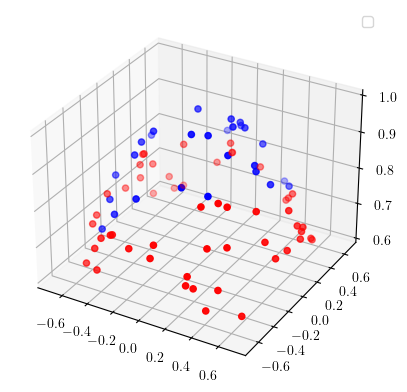
\includegraphics[width=.65\textwidth]{pics/vm-data-sphere-projection.png}
        \end{minipage}

        \pause
        \begin{minipage}{.45\textwidth}
            \centering
            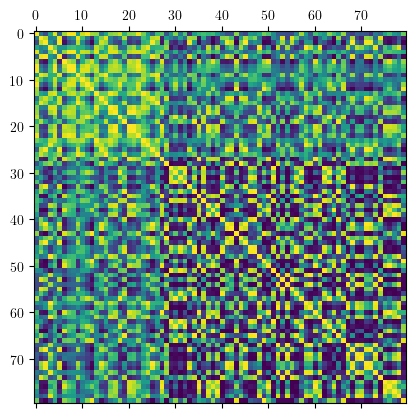
\includegraphics[width=.7\textwidth]{pics/amp-enc-sphere-kernel-matrix.png}
        \end{minipage}
        \begin{minipage}{.45\textwidth}
            \centering
            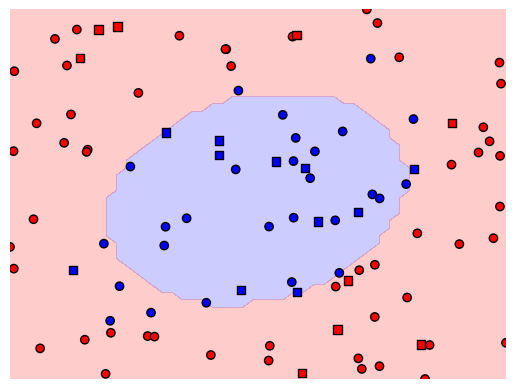
\includegraphics[width=.8\textwidth]{pics/amp-enc-sphere-envelope.png}
        \end{minipage}
        
    \end{frame}
    
    \begin{frame}
        \frametitle{Von Mises criterion}
        \framesubtitle{Rotation encoding kernels}

        \footnotesize
        Can we do better and avoid feature pre-processing that can confuse the label spaces?
        
        \begin{block}{\small Rotation encoding}
            \footnotesize
            Encode every feature as the rotation angle of a gate.

            \begin{minipage}{.45\textwidth}
                $\phi\left( \mathbf{x} \right) = R\left( x_1 \right)\otimes R\left( x_2 \right) \ket{0}^{\otimes 2}$
            \end{minipage}
            \begin{minipage}{.45\textwidth}
                \centering
                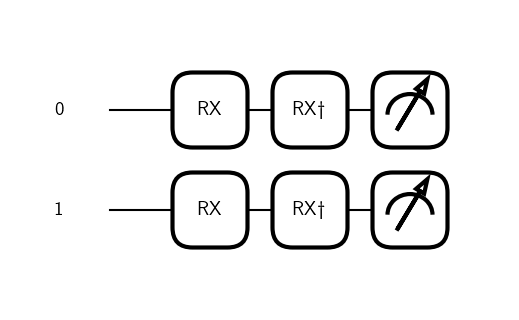
\includegraphics[width=.7\textwidth]{pics/rot-enc-circuit.png}
            \end{minipage}
        \end{block}

        \pause
        \begin{minipage}{.45\textwidth}
            \centering
            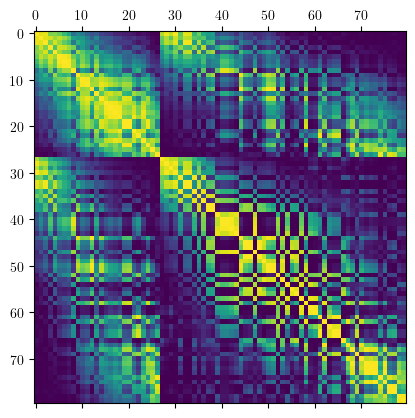
\includegraphics[width=.7\textwidth]{pics/rot-enc-kernel-matrix.png}
        \end{minipage}
        \begin{minipage}{.45\textwidth}
            \centering
            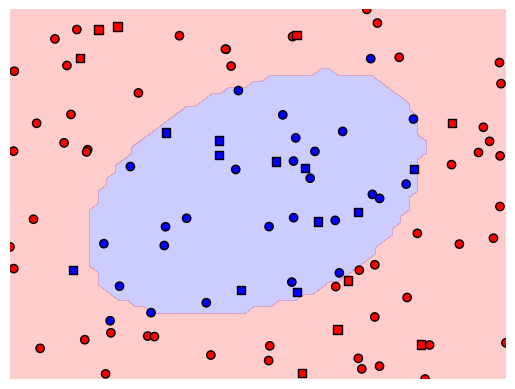
\includegraphics[width=.8\textwidth]{pics/rot-enc-kernel-envelope.png}
        \end{minipage}
        
        
    \end{frame}

    \begin{frame}
        \frametitle{Summary}
    
        Classifying stresses based on the Von Mises criterion has little direct interest, but
        \begin{enumerate}
            \pause
            \item It provides a reality-based example to compare the accuracies of classical and quantum kernels.
            \pause
            \item It highlights the key aspects of data encoding in quantum states
            \begin{itemize}
                \item normalization
                \item data scaling
                \item data dimensionality
            \end{itemize} 
        \end{enumerate}
    
    \end{frame}
    
    \begin{frame}
        \frametitle{Where to go from here}
        
        \begin{itemize}
            \item Study more complex datasets, where the `ground truth' is unknown
            \begin{itemize}
                \item Experimental data
                \item Numerical, high-fidelity data
            \end{itemize} 
            \pause
            \item Further investigate near-term encodings for damage prediction
            \begin{itemize}
                \item In particular, quantum kernels generated by Hamiltonian evolution ($e^{iH \mathbf{x}}$) correspond to Fourier series in the data
                $$
                    k\left( \mathbf{x}, \mathbf{x}^\prime \right) = \sum_{\mathbf{n}, \mathbf{n}^\prime \in \Omega} c_{\mathbf{n}, \mathbf{n}^\prime} e^{i \mathbf{n}\mathbf{x}} e^{i \mathbf{n}^\prime\mathbf{x}^\prime}
                $$
                
            \end{itemize}
            \pause
            \item Encode problem knowledge in the circuit to have control over the $c_{n_i,n_j}$ coefficients
            \begin{itemize}
                \item e.g. encoding symmetries \footnote{La Rocca \emph{et al.}, 2022, PRX Quantum} 
            \end{itemize}
        \end{itemize}
        
    \end{frame}
    
    \begin{frame}[noframenumbering]
        
        \centering
        Thank you!
        
        
    \end{frame}
    
    \begin{frame}[noframenumbering]
        \frametitle{Dual formulation of the maximum margin classifier}
        
        
        
    \end{frame}
    

    \begin{frame}[noframenumbering]
        \frametitle{Classical kernels}
    
        Some examples of classical kernels
    
    \end{frame}

    \begin{frame}[noframenumbering]
        \frametitle{Amplitude encoding circuits}
    
        2 qubits

        4 qubits
    
    \end{frame}

    \begin{frame}[noframenumbering]
        \frametitle{Single rotation kernel encoding for 2 qubits}
    
        
    
    \end{frame}
    % Equivalent to finding
    % \[
        %     \min_{w,b} \,\max_{i=1,\dots m} y^{(i)}\left( \left( \frac{\mathbf{w}}{\norm{\mathbf{w}}} \right)^\top \mathbf{x}^{(i)} + \frac{b}{\norm{\mathbf{w}}} \right)
        % \]
        
        
\end{document}
        